\documentclass{article}
\usepackage{graphicx}
\usepackage{indentfirst}
\usepackage{float}
\usepackage{caption}
\usepackage{pdfpages}
\usepackage{pdflscape}
\usepackage{amsmath}
\usepackage{url}
\usepackage{verbatim}
\usepackage[numbib,nottoc]{tocbibind}
\usepackage{tocloft} % Add the tocloft package

% Add dotted lines to the table of contents
\renewcommand{\cftsecleader}{\cftdotfill{\cftdotsep}} % Dotted lines for sections
\renewcommand{\cftsubsecleader}{\cftdotfill{\cftdotsep}} % Dotted lines for subsections

% -------Clickable Table of Contents ----------

\usepackage{color}   %May be necessary if you want to color links
\usepackage{hyperref}
\hypersetup{
    colorlinks=true, %set true if you want colored links
    linktoc=all,     %set to all if you want both sections and subsections linked
    linkcolor=blue,  %choose some color if you want links to stand out
}





\begin{document}

\begin{titlepage}
	\begin{center}
	\includegraphics[width=\textwidth,scale=0.25]{"TECH_Logo_Main_TransparentBkgd_Purple".png} \\
	[2mm]
	\textsc{\Large by cory stephenson} \\
	[0.75cm]
	\textsc{\Large met 3000: principles of metal casting} \\
	[0.75cm]
	\textsc{\Large dr. fred vondra} \\
	[0.75cm]
	\textsc{\Large april 5, 2017} \\
	[0.75cm]
	\textsc{\Large nobe casting}\\
	
	
	 \end{center}
        
\end{titlepage}

\tableofcontents
\thispagestyle{empty}
\cleardoublepage

\vfill
\begin{landscape}
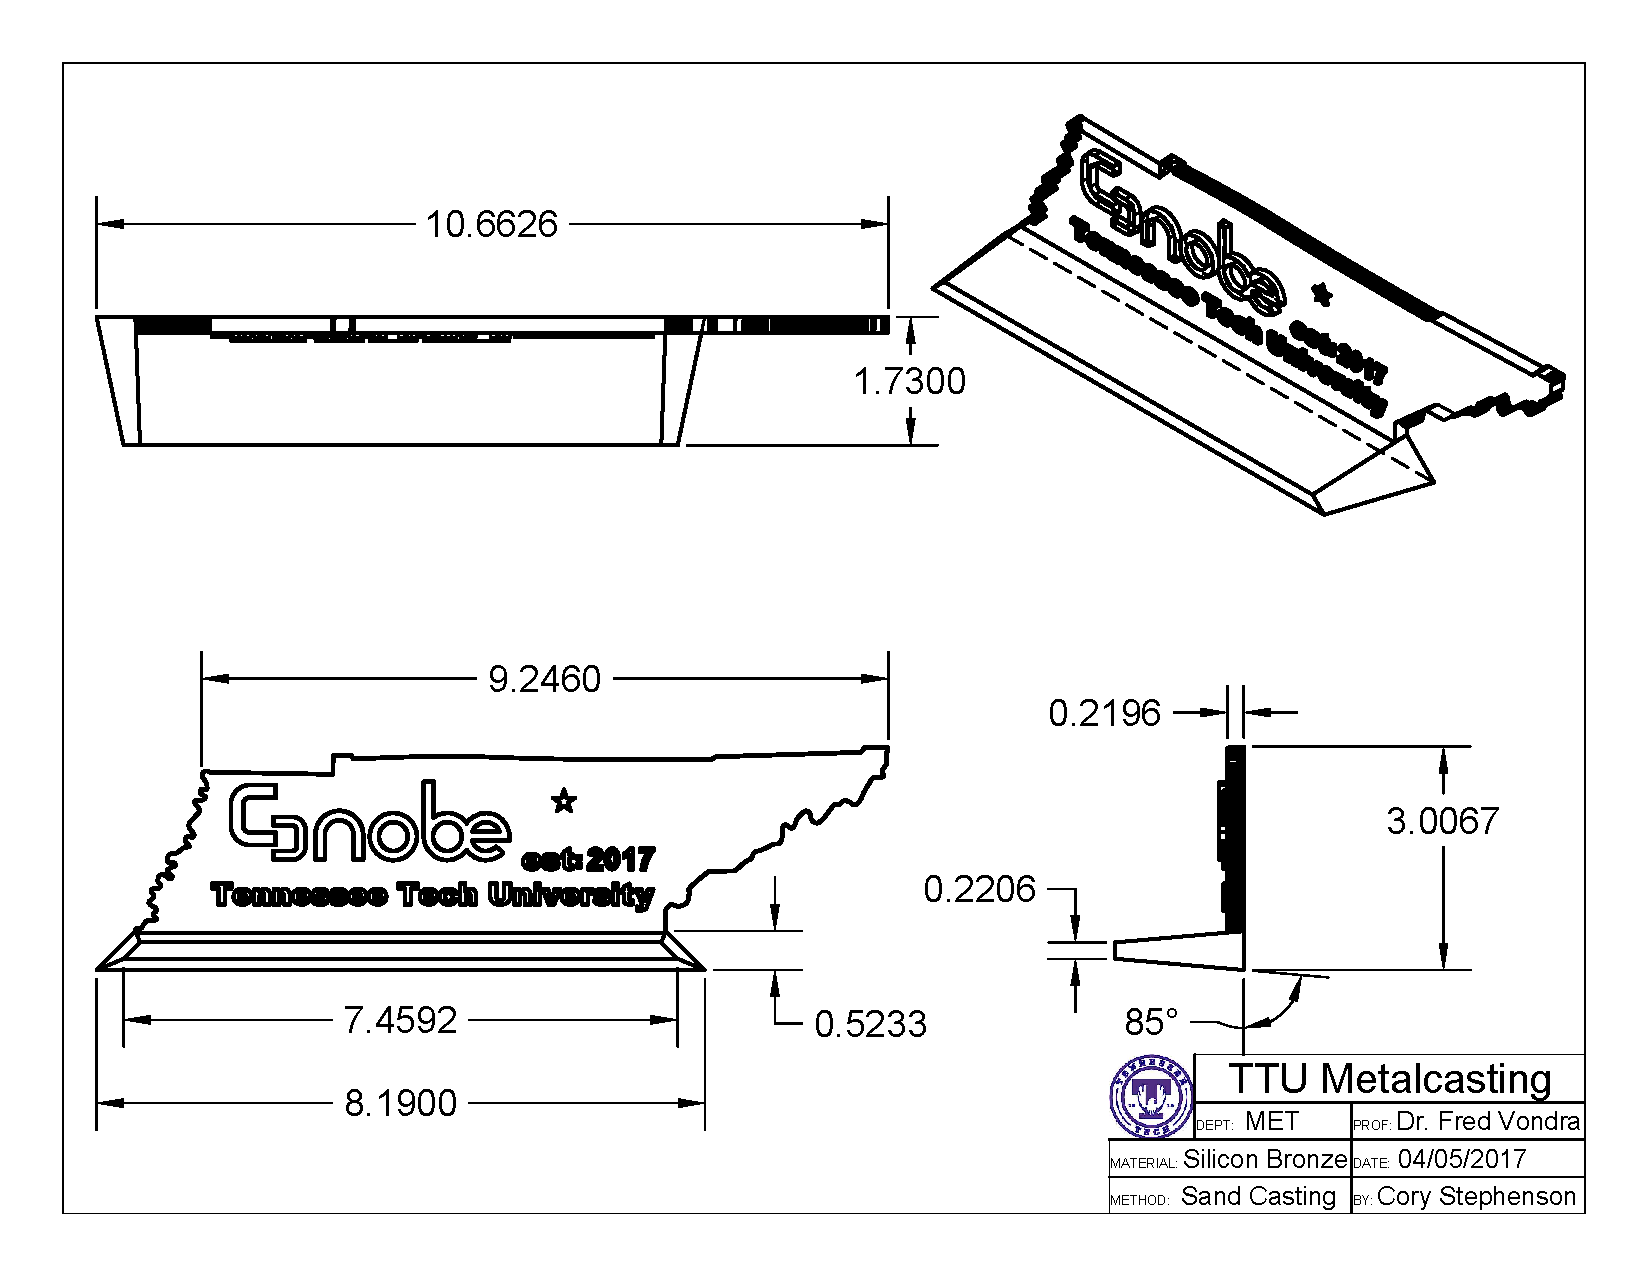
\includepdf[pages=1,pagecommand={\thispagestyle{empty}}, fitpaper=true]{NOBEcasting}
\includepdf[pages=1,pagecommand={\thispagestyle{empty}}, fitpaper=true]{Gates}
\end{landscape}

\section{Introduction & History}

It is my intention that this introduction will serve as a generalized mission
statement that outlines my motives behind the creation of the Tennessee Tech
chapter of the National Organization for Business & Engineering (NOBE). Any
business  starts  with  an  idea,  and  these  potentially  protable  ideas  can  come
from anyone,  whether they are a business professional or an engineering pro-
fessional.  The goal of the business professional is to monitor performance and
facilitate the acquisition of revenue.  The goal of the engineering professional is
to devise the most ecient, eective, reliable, economical, and desirable means
of achieving the goals laid out by the business professional.  This organization
merges the two goals into one.

I  was  encouraged  by  Dr.   Ismail  Fidan  of  the  Manufacturing  &  Engineer-
ing  Technology  department  and  Dr.   Brian  Nagy  of  the  Decision  Sciences  &
Management department to strengthen the relationship between the College of
Business and the College of Engineering.  It soon became evident to me that
the best way to accomplish this was to start a student organization.  Using the
knowledge and resources I had gained from a close friend of mine,  I unveiled
plans  to  form  a  cooperative  business  \incubator"  between  NOBE  and  Eagle-
works, TTU's innovation and entrepreneurship competition.

As  the  co-founder  and  nascent  president  of  the  local  student  chapter,  I
wanted this casting to symbolize our commitment and future contributions to
the university.  NOBE will play an instrumental role in the continuation of Ten-
nessee Tech's global reputation of excellence.  The pattern for the casting (that
you will see on the next page) was 3D printed in plastic.  The distinct outline of
the state of Tennessee forms the surface upon which the chapter's logo is em-
bossed, along with a small star that represents Cookeville.  Beneath Cookeville
is the year that the chapter was founded.  This pattern can be poured in either
aluminum, silicon bronze, or gray iron.  For the sake of this report, it was as-
sumed that the casting is to be poured in silicon bronze.

The technical drawings that were included in this report were rendered in
AutoCAD. A perspective drawing articulates every aspect of the casting's de-
sign,  including  features  and  accurate  dimensions.   In  addition,  every  vertical
surface was given a draft of 5%.The drawing is comprised of four views (coun-
terclockwise):  top view,  front view,  right-side view,  and isometric view.  The
gating system was also simulated with a separate drawing.  A traditional gating
system  (comprised  of  a  sprue,  runner  bar,  and  gates)  is  shown  because  it  is
easier to visualize.  However, it was brought to my attention that a matchplate
pattern might be more suitable for this casting.

\section{Casting Yield}

The casting yield, Y, is defined as the ratio of the actual casting weight, W, to the weight of metal poured into the mold, w, which includes the weight of the gating and risering system, and is expressed as follows (\%): \cite{LerRao} 

\begin{equation}
Y = \% \frac{W}{w} \times 100
\end{equation}

Generally, those casting alloys that shrink heavily have lower casting yields. Also, massive and simple shapes have higher casting yield, compared to small and complex parts. \cite{LerRao} 

In order to calculate the casting yield, the weights of both the NOBE casting and the gating system were found separately using the MASSPROPS (Volume) function in AutoCAD. Once the volumes of the two casting sections is found, the mass that corresponds to each of those volumes can be derived from the following equation.

\begin{equation}
D = \frac{m}{v}
\end{equation}

The density of Everdur Silicon Bronze, D, is $0.302\ \mathrm{{ lb_f }/{ in^3}}$ according to a data sheet from Belmont Metals Inc.\cite{BelMet} After rearranging the above equation so that mass could be solved for, the equation assumes the following form.

\begin{equation}
m = D \times v
\end{equation}



\begin{figure}[H]
\captionsetup{format =hang}
  \begin{minipage}[b]{0.4\textwidth}
    \includegraphics[width=\textwidth]{"NOBE Volume".png}
    \caption{Volume of NOBE casting}
    \label{fig:1}
  \end{minipage}
  \hfill
  \begin{minipage}[b]{0.4\textwidth}
    \includegraphics[width=\textwidth]{"Gates etc".png}
    \caption{Volume of gating\\ system}
    \label{fig:2}
  \end{minipage}
\end{figure}



\newpage


According to Figure \ref{fig:1}, the volume of the NOBE casting is taken to be equivalent to $9.0427\ \mathrm{in^3}$, which is rounded to $9.043\ \mathrm{in^3}$ for simplicity. Likewise, according to Figure \ref{fig:2}, the volume of the gating system is taken to be equivalent to $10.4404\ \mathrm{in^3}$, which is rounded to $10.44\ \mathrm{in^3}$. 

\begin{alignat}{2}
\frac{0.302\ \mathrm{lb_f}}{\mathrm{in^3}} \times 9.043\ \mathrm{in^3} = 2.731\ \mathrm{lb_f} \label{eq:4} \\[0.5cm] 
\qquad\frac{0.302\ \mathrm{lb_f}}{\mathrm{in^3}} \times 10.44\ \mathrm{in^3} = 3.153\ \mathrm{lb_f} \label{eq:5}
\end{alignat} 

The weight of the NOBE casting is shown in equation \eqref{eq:4}, while the weight of the gating system is shown in equation \eqref{eq:5}. Now, the casting yield can be calculated.

\begin{equation}
Y = \frac{2.731}{2.731 + 3.153} \times 100 = 46.41\ \%
\end{equation}
 
 
 
\section{Shrinkage Allowance}

The shrinkage calculation was carried out with a shrinkage allowance of 2\%, in accordance with the range of shrinkage values corresponding to bronze in the textbook. The volume of the NOBE casting given in Figure \ref{fig:1} is no longer accurate, due to the contraction of the casting as it cools and solidifies. This discrepancy is found via the following calculation.

\begin{equation}
9.0427\ \mathrm{in^3} \times (1 - .02) = 9.0427\ \mathrm{in^3} \times (0.98) = 8.86\ \mathrm{in^3} \label{eq:7}
\end{equation}

The volume that results from equation \eqref{eq:7} is the true volume of the casting. The casting is reduced to this overall volume after it is poured and subsequently undergoes solidification and cooling. In order for a given casting to meet the desired dimensional requirements, the amount of shrinkage that corresponds to the specified casting alloy has got to be figured prior to the pouring process. This allows the shrinkage to be compensated for.

\newpage



\section{Conclusion}

Although I still know very little about the metal casting industry, I now respect the trade more than ever. It is an art unto itself. Still, I am completely awestruck by the sheer scope of the subject matter. An extremely large portion of the products that we interact with each and every day were formed by any number of these exotic manufacturing processes. I had no idea that our way of life was so heavily reliant on such an intricate industry, not to mention the rich history that it has. Having completed this course, I now understand how important metal casting is as a class of manufacturing processes. Some of the products that we use throughout our lives cannot be formed by any other means.This fact alone is indicative of a substantial impact on the global economy.  

\begin{figure}[H]
\captionsetup{format =hang}
  \begin{minipage}[b]{0.4\textwidth}
    \includegraphics[width=\textwidth, angle=180]{"IMG_0749".jpg}
    \caption{3D printed pattern}
    \label{fig:1}
  \end{minipage}
  \hfill
  \begin{minipage}[b]{0.4\textwidth}
    \includegraphics[width=\textwidth]{"Cory Stephenson-Temp0001".png}
    \caption{Bronze rendering\\ in AutoCAD}
    \label{fig:2}
  \end{minipage}
\end{figure}



\section{Acknowledgements}


The results of this project would not have been possible if it wasn't for the efforts of Billy House and my professor, Dr. Vondra. Also, I would like to thank Hunter Hinshaw for assisting me in getting the pattern 3D printed. This NOBE chapter would not have made it this far if it wasn't for the faculty advisors and my fellow NOBE officers: Dr. Brian Nagy, Ms. Elizabeth Hutchins, Michael Sia, Madeleine Mae Reinke, Hayden Poirier, and Timothy McGovern. My appreciation again goes out to Seth Haynes for creating the NOBE logo, and to Mitchell Stooksbury for converting it to a vector file for me. Our future seems bright! To the students who participated in the preliminary meetings, your support is deeply appreciated as well. See you all next year!

\section{References}
  
\cleardoublepage
\begin{thebibliography}{9}
\bibitem{LerRao} Yury S. Lerner and P. N. Rao, \textit{Metalcasting Principles and Techniques}(Schaumburg, IL:American Foundry Society, 2013), 65.
\bibitem{BelMet} \textit{Everdur Silicon Bronze Product 4951}; SDS BB-3.1 [Online]; Belmont Metals Inc.:Brooklyn,NY,\url{<http://www.belmontmetals.com/wp-content/} \\
\url{uploads/2013/12/BB-3-1-Belmont-Everdur-4951.pdf>}

\end{thebibliography} 

\end{document}

